% Options for packages loaded elsewhere
\PassOptionsToPackage{unicode}{hyperref}
\PassOptionsToPackage{hyphens}{url}
%
\documentclass[
  man,floatsintext]{apa6}
\usepackage{amsmath,amssymb}
\usepackage{lmodern}
\usepackage{iftex}
\ifPDFTeX
  \usepackage[T1]{fontenc}
  \usepackage[utf8]{inputenc}
  \usepackage{textcomp} % provide euro and other symbols
\else % if luatex or xetex
  \usepackage{unicode-math}
  \defaultfontfeatures{Scale=MatchLowercase}
  \defaultfontfeatures[\rmfamily]{Ligatures=TeX,Scale=1}
\fi
% Use upquote if available, for straight quotes in verbatim environments
\IfFileExists{upquote.sty}{\usepackage{upquote}}{}
\IfFileExists{microtype.sty}{% use microtype if available
  \usepackage[]{microtype}
  \UseMicrotypeSet[protrusion]{basicmath} % disable protrusion for tt fonts
}{}
\makeatletter
\@ifundefined{KOMAClassName}{% if non-KOMA class
  \IfFileExists{parskip.sty}{%
    \usepackage{parskip}
  }{% else
    \setlength{\parindent}{0pt}
    \setlength{\parskip}{6pt plus 2pt minus 1pt}}
}{% if KOMA class
  \KOMAoptions{parskip=half}}
\makeatother
\usepackage{xcolor}
\usepackage{graphicx}
\makeatletter
\def\maxwidth{\ifdim\Gin@nat@width>\linewidth\linewidth\else\Gin@nat@width\fi}
\def\maxheight{\ifdim\Gin@nat@height>\textheight\textheight\else\Gin@nat@height\fi}
\makeatother
% Scale images if necessary, so that they will not overflow the page
% margins by default, and it is still possible to overwrite the defaults
% using explicit options in \includegraphics[width, height, ...]{}
\setkeys{Gin}{width=\maxwidth,height=\maxheight,keepaspectratio}
% Set default figure placement to htbp
\makeatletter
\def\fps@figure{htbp}
\makeatother
\setlength{\emergencystretch}{3em} % prevent overfull lines
\providecommand{\tightlist}{%
  \setlength{\itemsep}{0pt}\setlength{\parskip}{0pt}}
\setcounter{secnumdepth}{-\maxdimen} % remove section numbering
% Make \paragraph and \subparagraph free-standing
\ifx\paragraph\undefined\else
  \let\oldparagraph\paragraph
  \renewcommand{\paragraph}[1]{\oldparagraph{#1}\mbox{}}
\fi
\ifx\subparagraph\undefined\else
  \let\oldsubparagraph\subparagraph
  \renewcommand{\subparagraph}[1]{\oldsubparagraph{#1}\mbox{}}
\fi
\newlength{\cslhangindent}
\setlength{\cslhangindent}{1.5em}
\newlength{\csllabelwidth}
\setlength{\csllabelwidth}{3em}
\newlength{\cslentryspacingunit} % times entry-spacing
\setlength{\cslentryspacingunit}{\parskip}
\newenvironment{CSLReferences}[2] % #1 hanging-ident, #2 entry spacing
 {% don't indent paragraphs
  \setlength{\parindent}{0pt}
  % turn on hanging indent if param 1 is 1
  \ifodd #1
  \let\oldpar\par
  \def\par{\hangindent=\cslhangindent\oldpar}
  \fi
  % set entry spacing
  \setlength{\parskip}{#2\cslentryspacingunit}
 }%
 {}
\usepackage{calc}
\newcommand{\CSLBlock}[1]{#1\hfill\break}
\newcommand{\CSLLeftMargin}[1]{\parbox[t]{\csllabelwidth}{#1}}
\newcommand{\CSLRightInline}[1]{\parbox[t]{\linewidth - \csllabelwidth}{#1}\break}
\newcommand{\CSLIndent}[1]{\hspace{\cslhangindent}#1}
\ifLuaTeX
\usepackage[bidi=basic]{babel}
\else
\usepackage[bidi=default]{babel}
\fi
\babelprovide[main,import]{english}
% get rid of language-specific shorthands (see #6817):
\let\LanguageShortHands\languageshorthands
\def\languageshorthands#1{}
% Manuscript styling
\usepackage{upgreek}
\captionsetup{font=singlespacing,justification=justified}

% Table formatting
\usepackage{longtable}
\usepackage{lscape}
% \usepackage[counterclockwise]{rotating}   % Landscape page setup for large tables
\usepackage{multirow}		% Table styling
\usepackage{tabularx}		% Control Column width
\usepackage[flushleft]{threeparttable}	% Allows for three part tables with a specified notes section
\usepackage{threeparttablex}            % Lets threeparttable work with longtable

% Create new environments so endfloat can handle them
% \newenvironment{ltable}
%   {\begin{landscape}\centering\begin{threeparttable}}
%   {\end{threeparttable}\end{landscape}}
\newenvironment{lltable}{\begin{landscape}\centering\begin{ThreePartTable}}{\end{ThreePartTable}\end{landscape}}

% Enables adjusting longtable caption width to table width
% Solution found at http://golatex.de/longtable-mit-caption-so-breit-wie-die-tabelle-t15767.html
\makeatletter
\newcommand\LastLTentrywidth{1em}
\newlength\longtablewidth
\setlength{\longtablewidth}{1in}
\newcommand{\getlongtablewidth}{\begingroup \ifcsname LT@\roman{LT@tables}\endcsname \global\longtablewidth=0pt \renewcommand{\LT@entry}[2]{\global\advance\longtablewidth by ##2\relax\gdef\LastLTentrywidth{##2}}\@nameuse{LT@\roman{LT@tables}} \fi \endgroup}

% \setlength{\parindent}{0.5in}
% \setlength{\parskip}{0pt plus 0pt minus 0pt}

% Overwrite redefinition of paragraph and subparagraph by the default LaTeX template
% See https://github.com/crsh/papaja/issues/292
\makeatletter
\renewcommand{\paragraph}{\@startsection{paragraph}{4}{\parindent}%
  {0\baselineskip \@plus 0.2ex \@minus 0.2ex}%
  {-1em}%
  {\normalfont\normalsize\bfseries\itshape\typesectitle}}

\renewcommand{\subparagraph}[1]{\@startsection{subparagraph}{5}{1em}%
  {0\baselineskip \@plus 0.2ex \@minus 0.2ex}%
  {-\z@\relax}%
  {\normalfont\normalsize\itshape\hspace{\parindent}{#1}\textit{\addperi}}{\relax}}
\makeatother

% \usepackage{etoolbox}
\makeatletter
\patchcmd{\HyOrg@maketitle}
  {\section{\normalfont\normalsize\abstractname}}
  {\section*{\normalfont\normalsize\abstractname}}
  {}{\typeout{Failed to patch abstract.}}
\patchcmd{\HyOrg@maketitle}
  {\section{\protect\normalfont{\@title}}}
  {\section*{\protect\normalfont{\@title}}}
  {}{\typeout{Failed to patch title.}}
\makeatother

\usepackage{xpatch}
\makeatletter
\xapptocmd\appendix
  {\xapptocmd\section
    {\addcontentsline{toc}{section}{\appendixname\ifoneappendix\else~\theappendix\fi\\: #1}}
    {}{\InnerPatchFailed}%
  }
{}{\PatchFailed}
\keywords{emotion regulation, regulatory effort, effort discounting, registered report, emotion regulation choice, emotion regulation flexibility, electromyography\newline\indent Word count: 9432}
\usepackage{lineno}

\linenumbers
\usepackage{csquotes}
\usepackage{booktabs}
\usepackage{longtable}
\usepackage{array}
\usepackage{multirow}
\usepackage{wrapfig}
\usepackage{float}
\usepackage{colortbl}
\usepackage{pdflscape}
\usepackage{tabu}
\usepackage{threeparttable}
\usepackage{threeparttablex}
\usepackage[normalem]{ulem}
\usepackage{makecell}
\usepackage{xcolor}
\usepackage{setspace}\doublespacing
\usepackage[final]{pdfpages}
\usepackage{chngcntr}
\ifLuaTeX
  \usepackage{selnolig}  % disable illegal ligatures
\fi
\IfFileExists{bookmark.sty}{\usepackage{bookmark}}{\usepackage{hyperref}}
\IfFileExists{xurl.sty}{\usepackage{xurl}}{} % add URL line breaks if available
\urlstyle{same} % disable monospaced font for URLs
\hypersetup{
  pdftitle={Supplementary Material for the Registered Report: Estimating individual subjective values of emotion regulation strategies},
  pdfauthor={Christoph Scheffel,1, Josephine Zerna,1, Anne Gärtner1, Denise Dörfel1,2, \& Alexander Strobel1},
  pdflang={en-EN},
  pdfkeywords={emotion regulation, regulatory effort, effort discounting, registered report, emotion regulation choice, emotion regulation flexibility, electromyography},
  hidelinks,
  pdfcreator={LaTeX via pandoc}}

\title{Supplementary Material for the Registered Report: Estimating individual subjective values of emotion regulation strategies}
\author{Christoph Scheffel\textsuperscript{$\dagger{}$,1}, Josephine Zerna\textsuperscript{$\dagger{}$,1}, Anne Gärtner\textsuperscript{1}, Denise Dörfel\textsuperscript{1,2}, \& Alexander Strobel\textsuperscript{1}}
\date{}


\shorttitle{Supplementary Material}

\authornote{

The authors made the following contributions. Christoph Scheffel: Conceptualization, Methodology, Funding acquisition, Formal analysis, Investigation, Project administration, Software, Visualization, Writing - original draft preparation, Writing - review \& editing; Josephine Zerna: Conceptualization, Methodology, Funding acquisition, Investigation, Project administration, Software, Visualization, Writing - review \& editing; Anne Gärtner: Formal analysis, Writing - review \& editing; Denise Dörfel: Conceptualization, Writing - review \& editing; Alexander Strobel: Conceptualization, Methodology, Writing - review \& editing. \textsuperscript{$\dagger{}$} Christoph Scheffel and Josephine Zerna contributed equally to this work.

Correspondence concerning this article should be addressed to Christoph Scheffel, Zellescher Weg 17, 01069 Dresden, Germany. E-mail: \href{mailto:christoph_scheffel@tu-dresden.de}{\nolinkurl{christoph\_scheffel@tu-dresden.de}}

}

\affiliation{\vspace{0.5cm}\textsuperscript{1} Chair of Differential and Personality Psychology, Faculty of Psychology, Technische Universität Dresden, 01069 Dresden, Germany\\\textsuperscript{2} Center for Information Services and High Performance Computing, Technische Universität Dresden, 01069 Dresden, Germany}

\begin{document}
\maketitle

\hypertarget{DesignTable}{%
\subsection{Design Table}\label{DesignTable}}

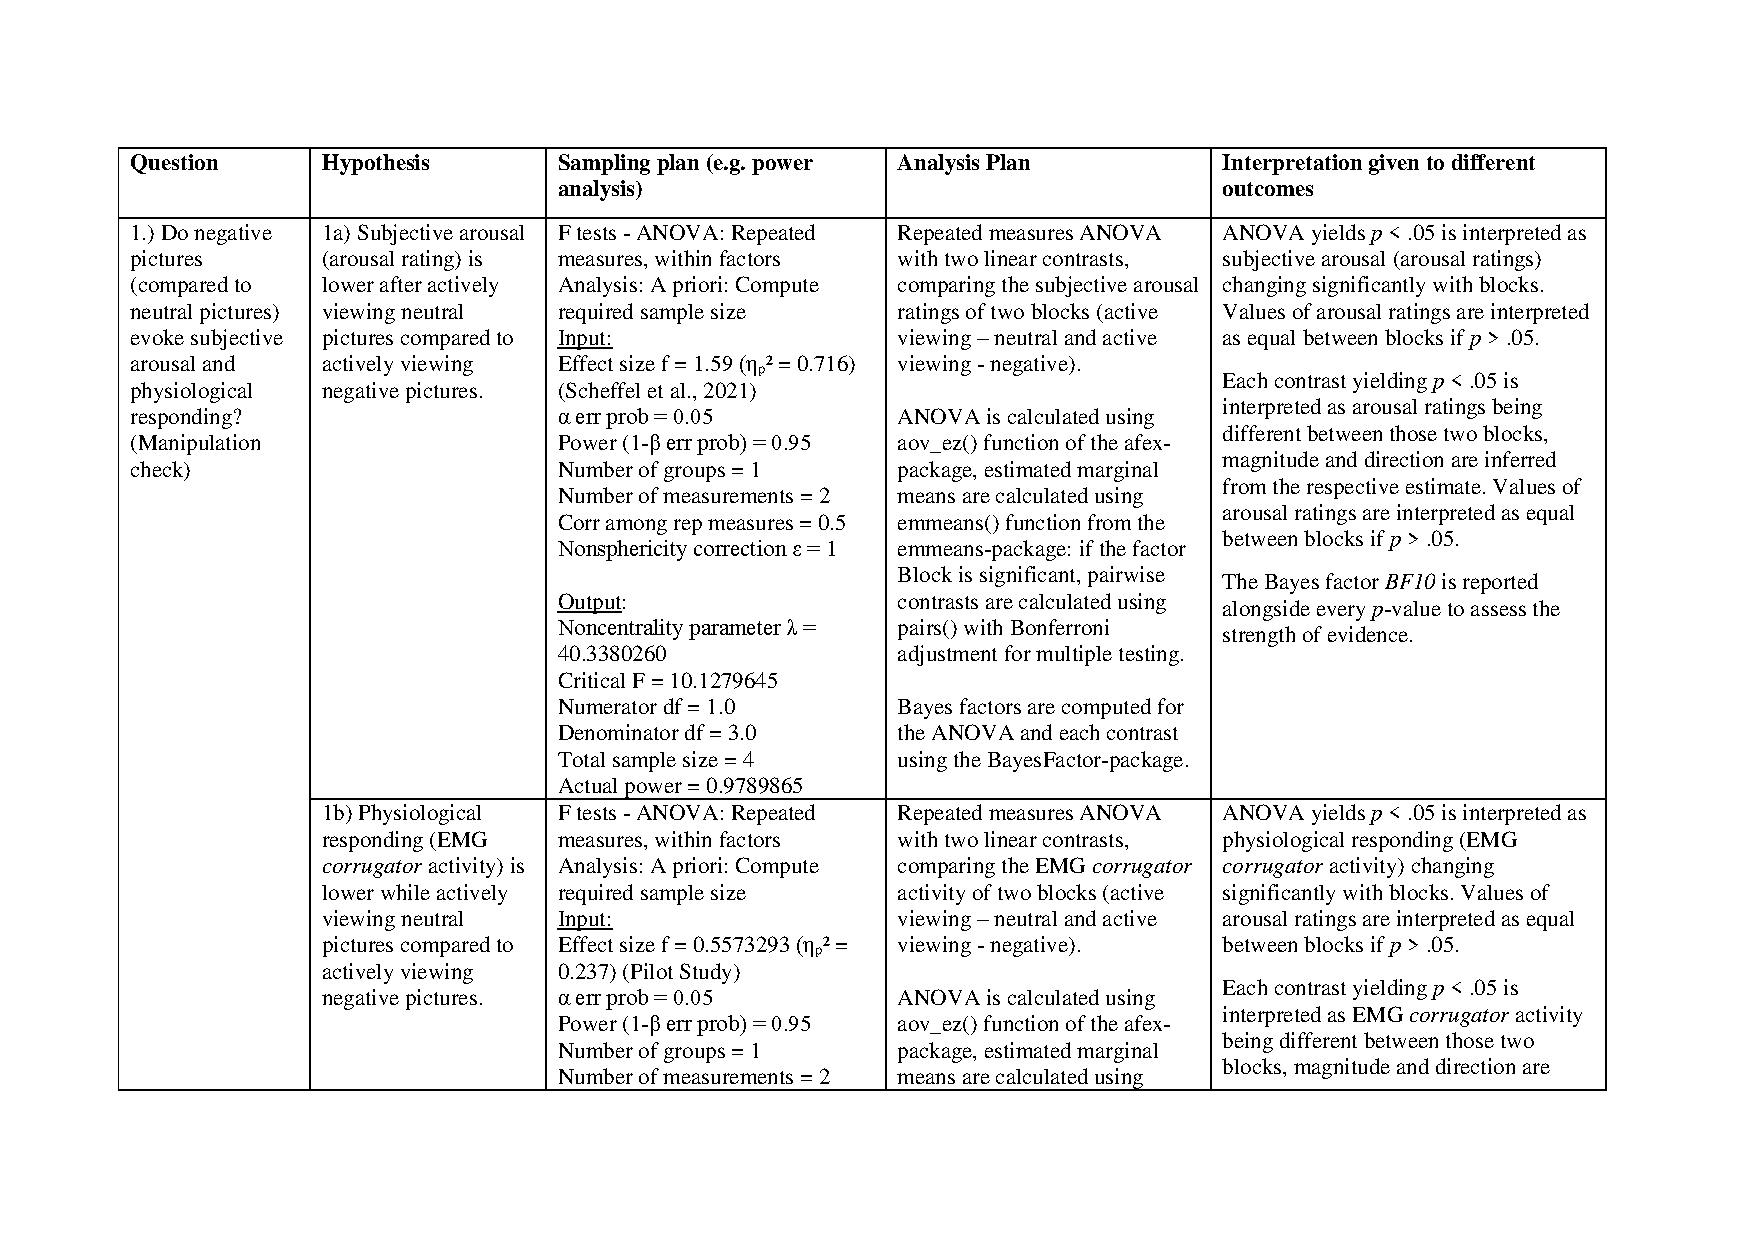
\includepdf[pages={-}, landscape=true]{Supplement/Design_Table_T2.pdf}
\newpage

\hypertarget{stimuli-used-in-er-paradigm}{%
\subsection{Stimuli used in ER paradigm}\label{stimuli-used-in-er-paradigm}}

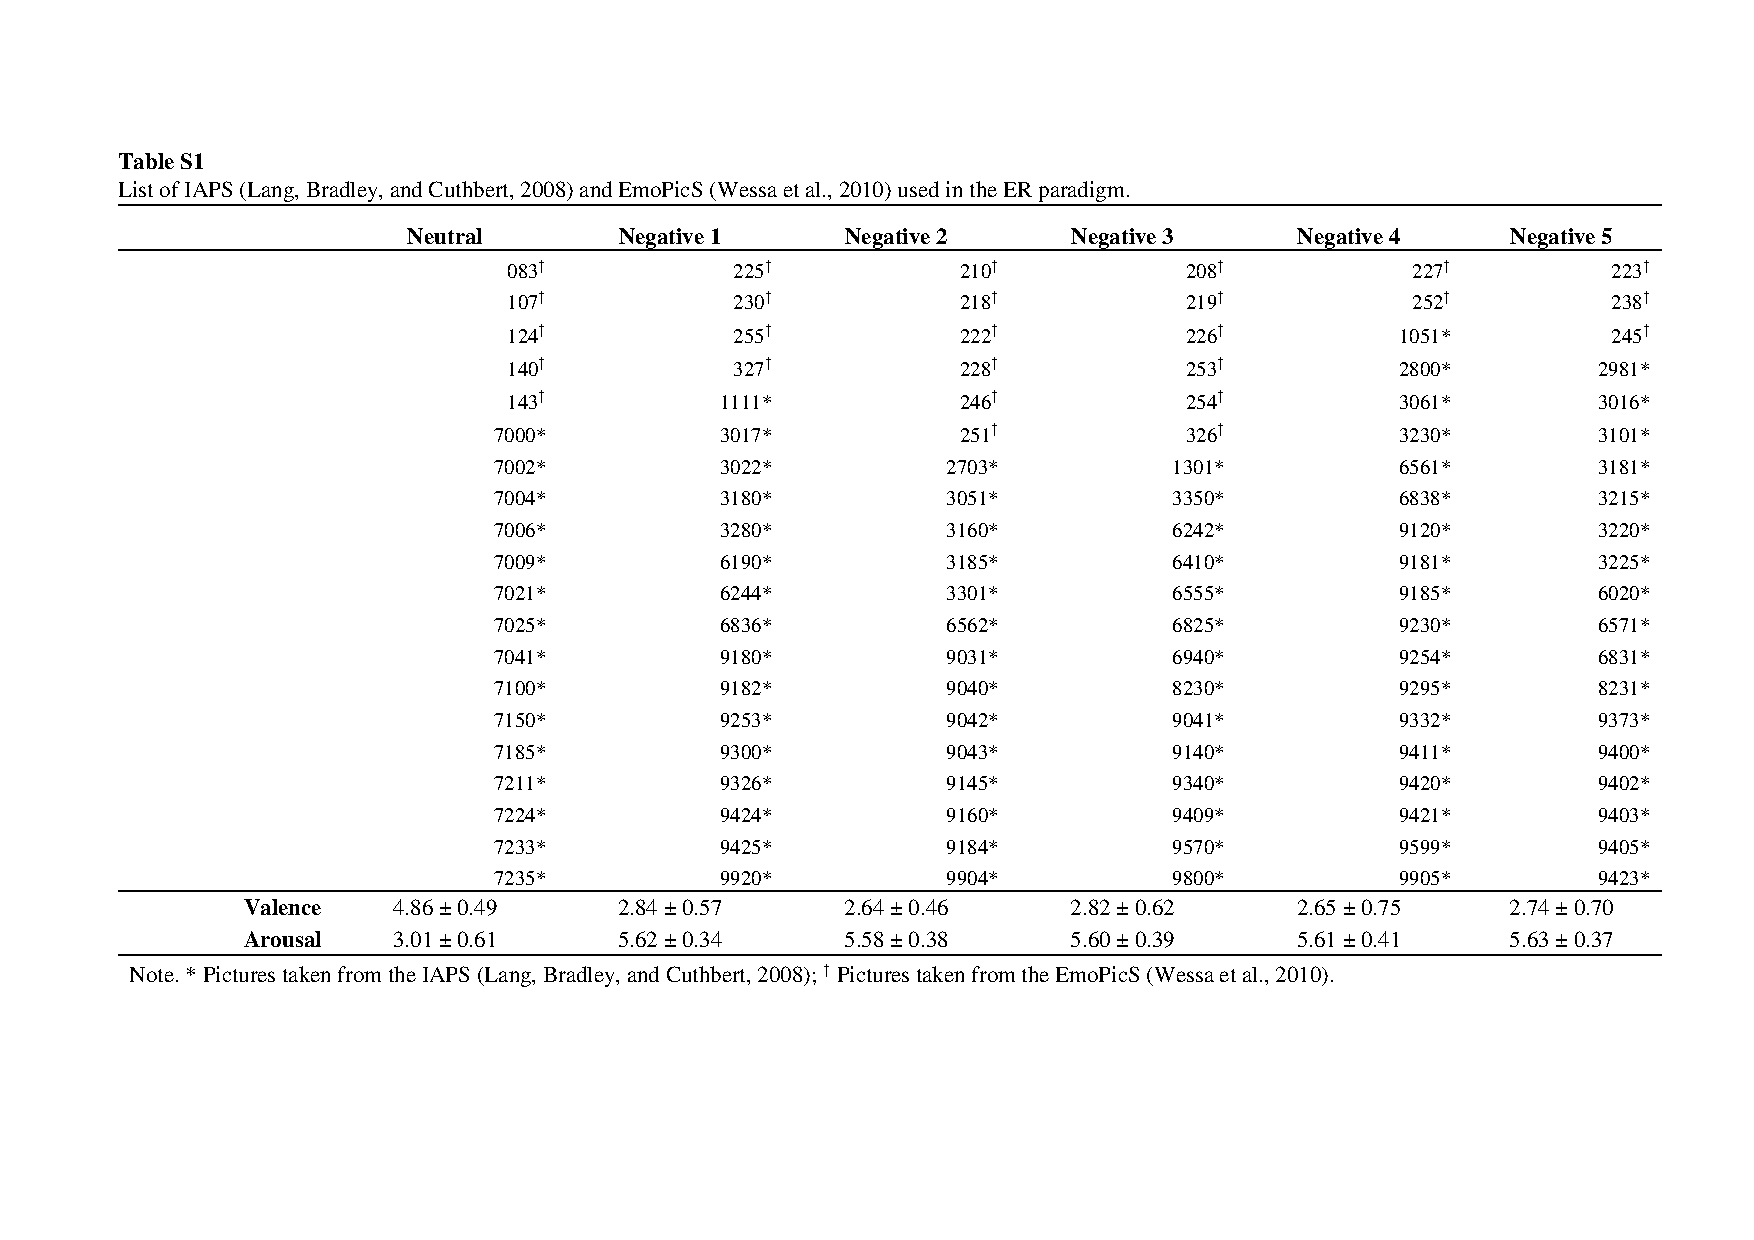
\includepdf[pages={-}, landscape=true]{Supplement/StimList_Suppl.pdf}

\renewcommand\thesection{\Alph{section}}
\counterwithin{figure}{section}
\counterwithin{table}{section}
\setcounter{section}{19}
\setcounter{figure}{0}
\setcounter{table}{1}
\newpage

\hypertarget{SupplementQuestionnaires}{%
\subsection{Detailed information on psychometric measures}\label{SupplementQuestionnaires}}

\emph{WHO-5.} General psychological well-being was assessed using the WHO-5 scale\textsuperscript{1,2}.
Five items such as ``Over the past 2 weeks I have felt calm and relaxed.'' are rated on a 6-point Likert scale raning from 0 (at no time) to 5 (all of the time).
The German version of the scale showed a high internal consistency (Cronbach's \(\alpha=.92\))\textsuperscript{2}.

\emph{Connor-Davidson Resilience Scale.} Resilience was assessed using the Connor-Davidson Resilience Scale (CD-RISC)\textsuperscript{3--5}.
Ten items such as ``I am able to adapt to change.'' are rated on a scale from 0 (not true at all) to 4 (true nearly all the time).
The 10-item version showed a high internal consistency (Cronbach's \(\alpha=.84\)) and a satisfactory retest-reliability of \(r_{tt}=.81\) across 6 months\textsuperscript{5}.

\emph{Emotion Regulation Questionnaire.} Habitual use of reappraisal and suppression was measured using the 10-item Emotion Regulation Questionnaire (ERQ)\textsuperscript{6,7}.
The scale has items such as ``I keep my emotions to myself'' (ERQ-suppression - 4 items) and ``When I'm faced with a stressful situation, I make myself think about it in a way that helps me stay calm'' (ERQ-reappraisal - 6 items), which are answered on a 7-point Likert scale ranging from 1 (strongly disagree) to 7 (strongly agree), and has acceptable to high internal consistency (Cronbach's \(\alpha>.75\))\textsuperscript{8}.

\emph{FlexER Scale.} Flexible use of ER strategies is assessed using the FlexER Scale\textsuperscript{9} with items such as ``If I want to feel less negative emotions, I have several strategies to achieve this.'', which are answered on a 4-point scale ranging from ``strongly agree'' to ``strongly disagree''.
Psychometric properties are currently under investigation.

\emph{Implicit Theories Questionnaire.} Implicit theories of willpower in emotional control were assessed using the Implicit Theories Questionnaire of Bernecker and Job\textsuperscript{10}.
Four items such as ``Having to control a strong emotion makes you exhausted and you are less able to manage your feelings right afterwards.'' are rated on a 6-point scale ranging from 1 (fully agree) to 6 (do not agree at all).
The questionnaire showed an internal consistency of Cronbach's \(\alpha=.87\)\textsuperscript{10}.

\emph{Need for Cognition Scale.} Need for Cognition (NFC) was assessed with the 16-item short version of the German NFC scale\textsuperscript{11}.
Responses to each item (e.g., ``Thinking is not my idea of fun'', recoded) are recorded on a 7-point Likert scale ranging from -3 (completely disagree) to +3 (completely agree) and are summed to the total NFC score.
The scale shows comparably high internal consistency (Cronbach's \(\alpha>.80\))\textsuperscript{11,12} and a retest reliability of \(r_{tt}=.83\) across 8 to 18 weeks\textsuperscript{13}.

\emph{Self-Regulation Scale.} As one measure of self-control, the Self-Regulation Scale (SRS)\textsuperscript{14} was used. The scale has 10 items (e.g., ``It is difficult for me to suppress thoughts that interfere with what I need to do.'', recoded) on a 4-point scale ranging from 1 (not at all true) to 4 (exactly true).
It has high internal consistency (Cronbach's \(\alpha>.80\))\textsuperscript{14}.

\emph{Brief Self-Control Scale.} As a second measure of self-control, the Brief Self-Control Scale (BSCS)\textsuperscript{15,16} was used.
It comprises 13 items (e.g., ``I am good at resisting temptations'') with a 5-point rating scale ranging from 1 (not at all like me) to 5 (very much like me).
The scale shows acceptable internal consistency (Cronbach's \(\alpha=.81\))\textsuperscript{16}.

\emph{Barratt Impulsiveness Scale.} As a third measure of self-control, the Barratt Impulsiveness Scale (BIS-11)\textsuperscript{17,18} was used.
Responses to each item (e.g., ``I am self-controlled.'', recoded) are assessed on a 4-point scale ranging from 1 (never/rarely) to 4 (almost always/always).
An internal consistency of Cronbach's \(\alpha=.74\) and a retest reliability of \(r_{tt}=.56\) for General Impulsiveness and \(r_{tt}=.66\) for Total Score across 6 month were reported\textsuperscript{18}.

\emph{Attentional Control Scale.} Attentional control was measured using the Attentional Control Scale (ACS)\textsuperscript{19} with items such as ``My concentration is good even if there is music in the room around me''.
The 20 items are rated on a 4-point scale ranging from 1 (almost never) to 4 (always).
An internal consistency of Cronbach's \(\alpha=.88\) was reported\textsuperscript{19}.

\newpage

\hypertarget{SupplementNV}{%
\subsection{Test for normal distribution of predictor variables}\label{SupplementNV}}

\begin{table}[H]

\begin{center}
\begin{threeparttable}

\caption{\label{tab:TabNVRatings}Results of Shapiro-Wilk test for normal distribution of subjective arousal and effort ratings for all strategies.}

\begin{tabular}{lllll}
\toprule
 & \multicolumn{1}{c}{$M$} & \multicolumn{1}{c}{$SD$} & \multicolumn{1}{c}{$W$} & \multicolumn{1}{c}{$p$}\\
\midrule
Arousal View Neu & 26.629 & 39.116 & 0.677 & <.001\\
Arousal View Neg & 187.778 & 87.308 & 0.979 & 0.057\\
Arousal Distraction & 158.129 & 92.492 & 0.972 & 0.014\\
Arousal Distancing & 168.617 & 95.754 & 0.978 & 0.043\\
Arousal Suppression & 163.957 & 87.165 & 0.980 & 0.073\\
Effort View Neu & 18.147 & 27.372 & 0.651 & <.001\\
Effort View Neg & 49.396 & 62.262 & 0.740 & <.001\\
Effort Distraction & 208.465 & 96.149 & 0.983 & 0.132\\
Effort Distancing & 158.259 & 99.505 & 0.969 & 0.007\\
Effort Suppression & 189.800 & 92.338 & 0.983 & 0.123\\
\bottomrule
\end{tabular}

\end{threeparttable}
\end{center}

\end{table}

\begin{table}[H]

\begin{center}
\begin{threeparttable}

\caption{\label{tab:TabNCEMG}Results of Shapiro-Wilk test for normal distribution of Corrugator and Levator activity for all strategies.}

\begin{tabular}{lllll}
\toprule
 & \multicolumn{1}{c}{$M$} & \multicolumn{1}{c}{$SD$} & \multicolumn{1}{c}{$W$} & \multicolumn{1}{c}{$p$}\\
\midrule
Corrugator View Neu & 0.041 & 6.991 & 0.046 & <.001\\
Corrugator View Neg & 1.030 & 7.213 & 0.194 & <.001\\
Corrugator Distraction & 0.004 & 7.668 & 0.040 & <.001\\
Corrugator Distancing & 0.066 & 3.784 & 0.083 & <.001\\
Corrugator Suppression & 0.246 & 1.924 & 0.354 & <.001\\
Levator View Neu & 0.090 & 1.838 & 0.384 & <.001\\
Levator View Neg & 0.580 & 3.198 & 0.429 & <.001\\
Levator Distraction & -0.050 & 1.157 & 0.520 & <.001\\
Levator Distancing & -0.027 & 0.917 & 0.481 & <.001\\
Levator Suppression & 0.010 & 0.996 & 0.554 & <.001\\
\bottomrule
\end{tabular}

\end{threeparttable}
\end{center}

\end{table}

\newpage

\hypertarget{SupplementEffectValence}{%
\subsection{Post-hoc contrasts for effects of valence on subjective arousal and physiological responding}\label{SupplementEffectValence}}

\begin{table}[H]

\begin{center}
\begin{threeparttable}

\caption{\label{tab:SupplEffectArousalView}Post-hoc contrasts for effects of valence on subjective arousal ratings in the active viewing conditions.}

\footnotesize{

\begin{tabular}{lllllllll}
\toprule
Contrast & \multicolumn{1}{c}{Estimate} & \multicolumn{1}{c}{$SE$} & \multicolumn{1}{c}{$df$} & \multicolumn{1}{c}{$t$} & \multicolumn{1}{c}{$p$} & \multicolumn{1}{c}{$\mathrm{BF}_{\textrm{10}}$} & \multicolumn{1}{c}{$\eta_{p}^{2}$} & \multicolumn{1}{c}{$95\% CI$}\\
\midrule
$View_{neutral} - View_{negative}$ & -161.15 & 8.06 & 119.00 & -20.00 & <.001 & $3.22 \times 10^{36}$ & 0.77 & {}[0.72, 1.00]\\
\bottomrule
\end{tabular}

}

\end{threeparttable}
\end{center}

\end{table}

\begin{figure}[H]
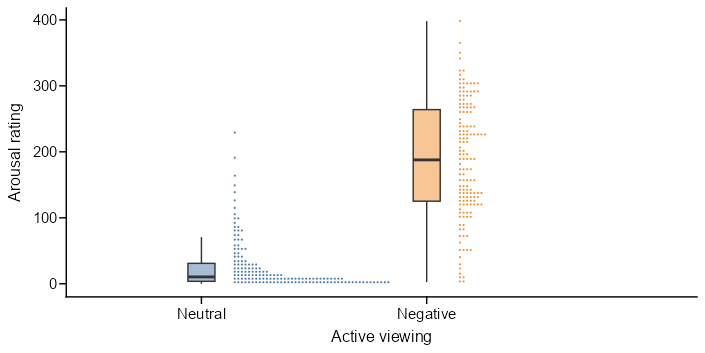
\includegraphics[width=\textwidth]{figures/FigSubjArousalView} \caption{Subjective arousal ratings of the active viewing conditions visualized as boxplots. Dots represent individual effort ratings placed in 150 quantiles.}\label{fig:SupplFigArousalView}
\end{figure}

\begin{table}[H]

\begin{center}
\begin{threeparttable}

\caption{\label{tab:SupplEffectCorrView}Post-hoc contrasts for effects of valence on Corrugator activity in the active viewing conditions.}

\footnotesize{

\begin{tabular}{lllllllll}
\toprule
Contrast & \multicolumn{1}{c}{Estimate} & \multicolumn{1}{c}{$SE$} & \multicolumn{1}{c}{$df$} & \multicolumn{1}{c}{$t$} & \multicolumn{1}{c}{$p$} & \multicolumn{1}{c}{$\mathrm{BF}_{\textrm{10}}$} & \multicolumn{1}{c}{$\eta_{p}^{2}$} & \multicolumn{1}{c}{$95\% CI$}\\
\midrule
$View_{neutral} - View_{negative}$ & -0.27 & 0.05 & 117.00 & -5.27 & <.001 & $8.67 \times 10^{16}$ & 0.19 & {}[0.10, 1.00]\\
\bottomrule
\end{tabular}

}

\end{threeparttable}
\end{center}

\end{table}

\begin{figure}[H]
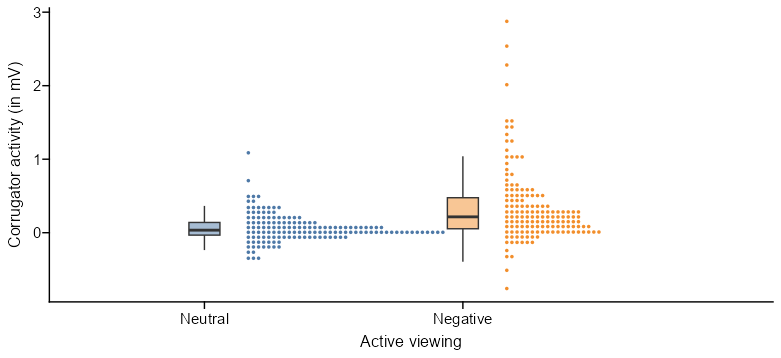
\includegraphics[width=\textwidth]{figures/FigCorrView} \caption{Corrugator activity in mV during the active viewing conditions, visualized as boxplots. Dots represent individual Corrugator activity measures placed in 150 quantiles.}\label{fig:SupplFigCorrView}
\end{figure}

\begin{table}[H]

\begin{center}
\begin{threeparttable}

\caption{\label{tab:SupplEffectLevView}Post-hoc contrasts for effects of valence on Levator activity in the active viewing conditions.}

\footnotesize{

\begin{tabular}{lllllllll}
\toprule
Contrast & \multicolumn{1}{c}{Estimate} & \multicolumn{1}{c}{$SE$} & \multicolumn{1}{c}{$df$} & \multicolumn{1}{c}{$t$} & \multicolumn{1}{c}{$p$} & \multicolumn{1}{c}{$\mathrm{BF}_{\textrm{10}}$} & \multicolumn{1}{c}{$\eta_{p}^{2}$} & \multicolumn{1}{c}{$95\% CI$}\\
\midrule
$View_{neutral} - View_{negative}$ & -0.23 & 0.08 & 117.00 & -2.98 & <.001 & 188.72 & 0.07 & {}[0.01, 1.00]\\
\bottomrule
\end{tabular}

}

\end{threeparttable}
\end{center}

\end{table}

\begin{figure}[H]
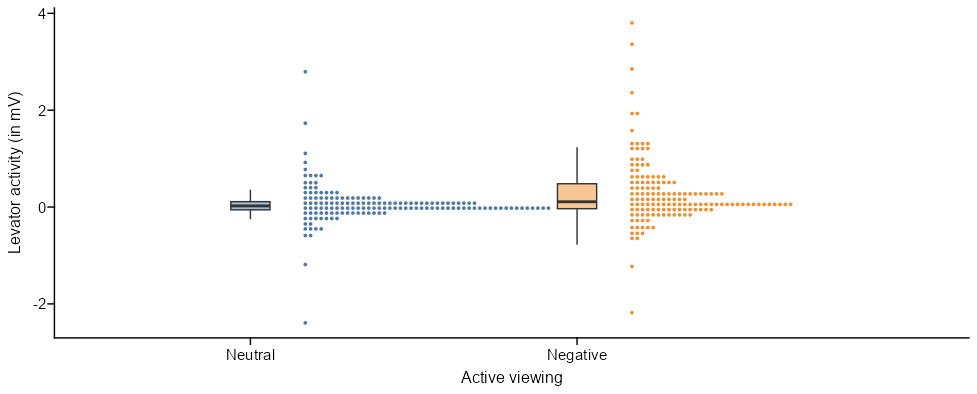
\includegraphics[width=\textwidth]{figures/FigLevView} \caption{Levator activity in mV during the active viewing conditions, visualized as boxplots. Dots represent individual Levator activity measures placed in 150 quantiles.}\label{fig:SupplFigLevView}
\end{figure}

\newpage

\hypertarget{SupplementEffectER}{%
\subsection{Post-hoc contrasts for effects of ER strategies on subjective arousal and physiological responding}\label{SupplementEffectER}}

\begin{table}[H]

\begin{center}
\begin{threeparttable}

\caption{\label{tab:SupplEffectArousalReg}Post-hoc contrasts for effects of ER strategies on subjective arousal ratings.}

\footnotesize{

\begin{tabular}{lllllllll}
\toprule
Contrast & \multicolumn{1}{c}{Estimate} & \multicolumn{1}{c}{$SE$} & \multicolumn{1}{c}{$df$} & \multicolumn{1}{c}{$t$} & \multicolumn{1}{c}{$p$} & \multicolumn{1}{c}{$BF10$} & \multicolumn{1}{c}{$\eta_{p}^{2}$} & \multicolumn{1}{c}{$95\% CI$}\\
\midrule
$View_{neg} - Distraction$ & 29.649 & 6.680 & 357.000 & 4.439 & 0.000 & 168.484 & 0.05 & {}[0.02, 1.00]\\
$View_{neg} - Distancing$ & 23.820 & 6.680 & 357.000 & 3.566 & 0.002 & 62.990 & 0.03 & {}[0.01, 1.00]\\
$View_{neg} - Suppression$ & 19.161 & 6.680 & 357.000 & 2.869 & 0.026 & 1.965 & 0.02 & {}[0.00, 1.00]\\
$Distraction - Distancing$ & -5.828 & 6.680 & 357.000 & -0.873 & 1.000 & 0.179 & 2.13e-03 & {}[0.00, 1.00]\\
$Distraction - Suppression$ & -10.488 & 6.680 & 357.000 & -1.570 & 0.704 & 0.309 & 6.86e-03 & {}[0.00, 1.00]\\
$Distancing - Suppression$ & -4.659 & 6.680 & 357.000 & -0.698 & 1.000 & 0.135 & 1.36e-03 & {}[0.00, 1.00]\\
\bottomrule
\end{tabular}

}

\end{threeparttable}
\end{center}

\end{table}

\begin{figure}[H]
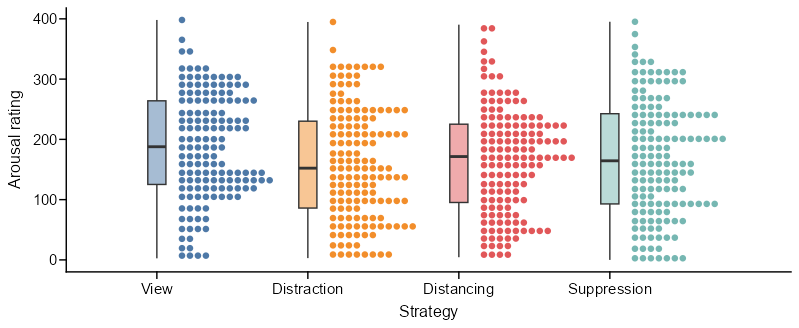
\includegraphics[width=\textwidth]{figures/FigSubjArousalReg} \caption{Subjective arousal ratings visualized as boxplots. Dots represent individual effort ratings placed in 150 quantiles.}\label{fig:SupplFigArousalReg}
\end{figure}

\begin{table}[H]

\begin{center}
\begin{threeparttable}

\caption{\label{tab:SupplEffectCorrReg}Post-hoc contrasts for effects of ER strategies on Corrugator activity}

\footnotesize{

\begin{tabular}{lllllllll}
\toprule
Contrast & \multicolumn{1}{c}{Estimate} & \multicolumn{1}{c}{$SE$} & \multicolumn{1}{c}{$df$} & \multicolumn{1}{c}{$t$} & \multicolumn{1}{c}{$p$} & \multicolumn{1}{c}{$BF10$} & \multicolumn{1}{c}{$\eta_{p}^{2}$} & \multicolumn{1}{c}{$95\% CI$}\\
\midrule
$View_{neg} - Distraction$ & 0.178 & 0.037 & 351.000 & 4.788 & 0.000 & 21,919.73 & 0.06 & {}[0.03, 1.00]\\
$View_{neg} - Distancing$ & 0.189 & 0.037 & 351.000 & 5.091 & 0.000 & 139,814.01 & 0.07 & {}[0.03, 1.00]\\
$View_{neg} - Suppression$ & 0.210 & 0.037 & 351.000 & 5.669 & 0.000 & $1.84 \times 10^{7}$ & 0.08 & {}[0.04, 1.00]\\
$Distraction - Distancing$ & 0.011 & 0.037 & 351.000 & 0.303 & 1.000 & $3.77 \times 10^{-2}$ & 2.61e-04 & {}[0.00, 1.00]\\
$Distraction - Suppression$ & 0.033 & 0.037 & 351.000 & 0.881 & 1.000 & $8.02 \times 10^{-2}$ & 2.21e-03 & {}[0.00, 1.00]\\
$Distancing - Suppression$ & 0.021 & 0.037 & 351.000 & 0.578 & 1.000 & $4.79 \times 10^{-2}$ & 9.51e-04 & {}[0.00, 1.00]\\
\bottomrule
\end{tabular}

}

\end{threeparttable}
\end{center}

\end{table}

\begin{figure}[H]
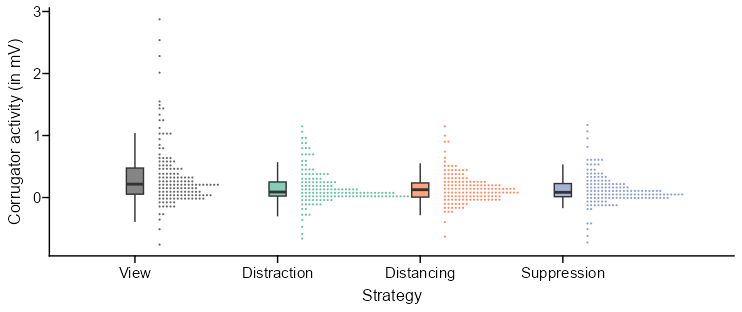
\includegraphics[width=\textwidth]{figures/FigCorrReg} \caption{Corrugator activity in mV visualized as boxplots. Dots represent individual Levatorr activity measures placed in 150 quantiles.}\label{fig:SupplFigCorrReg}
\end{figure}

\begin{table}[H]

\begin{center}
\begin{threeparttable}

\caption{\label{tab:SupplEffectLevReg}Post-hoc contrasts for effects of ER strategies on Levator activity}

\footnotesize{

\begin{tabular}{lllllllll}
\toprule
Contrast & \multicolumn{1}{c}{Estimate} & \multicolumn{1}{c}{$SE$} & \multicolumn{1}{c}{$df$} & \multicolumn{1}{c}{$t$} & \multicolumn{1}{c}{$p$} & \multicolumn{1}{c}{$BF10$} & \multicolumn{1}{c}{$\eta_{p}^{2}$} & \multicolumn{1}{c}{$95\% CI$}\\
\midrule
$View_{neg} - Distraction$ & 0.336 & 0.050 & 351.000 & 6.731 & 0.000 & $2.02 \times 10^{11}$ & 0.11 & {}[0.07, 1.00]\\
$View_{neg} - Distancing$ & 0.282 & 0.050 & 351.000 & 5.659 & 0.000 & $3.99 \times 10^{7}$ & 0.08 & {}[0.04, 1.00]\\
$View_{neg} - Suppression$ & 0.318 & 0.050 & 351.000 & 6.370 & 0.000 & $8.60 \times 10^{10}$ & 0.10 & {}[0.06, 1.00]\\
$Distraction - Distancing$ & -0.053 & 0.050 & 351.000 & -1.072 & 1.000 & 0.22 & 3.26e-03 & {}[0.00, 1.00]\\
$Distraction - Suppression$ & -0.018 & 0.050 & 351.000 & -0.361 & 1.000 & $3.91 \times 10^{-2}$ & 3.70e-04 & {}[0.00, 1.00]\\
$Distancing - Suppression$ & 0.035 & 0.050 & 351.000 & 0.711 & 1.000 & $9.86 \times 10^{-2}$ & 1.44e-03 & {}[0.00, 1.00]\\
\bottomrule
\end{tabular}

}

\end{threeparttable}
\end{center}

\end{table}

\begin{figure}[H]
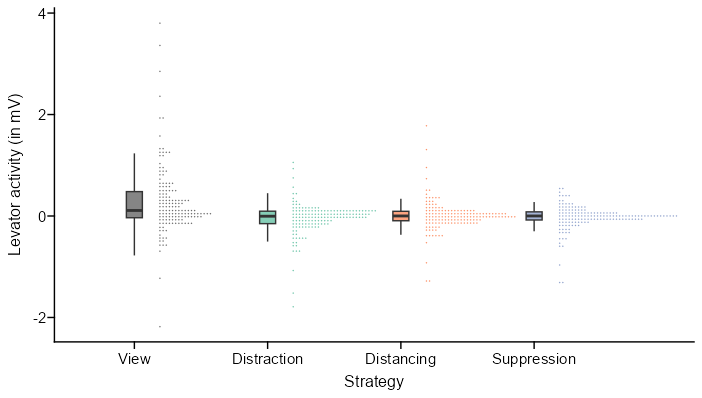
\includegraphics[width=\textwidth]{figures/FigLevReg} \caption{Levator activity in mV visualized as boxplots. Dots represent individual Levator activity measures placed in 150 quantiles.}\label{fig:SupplFigLevReg}
\end{figure}

\newpage

\hypertarget{exploratory-analysis-association-between-svs-and-self-control-and-nfc}{%
\subsection{Exploratory analysis: Association between SVs and self-control and NFC}\label{exploratory-analysis-association-between-svs-and-self-control-and-nfc}}

\begin{table}[H]

\begin{center}
\begin{threeparttable}

\caption{\label{tab:TabExp}Exploratory analysis: Results of MLM predicting SVs of ER strategies with level 2 predictors self-control and NFC.}

\begin{tabular}{llllll}
\toprule
Parameter & \multicolumn{1}{c}{Beta} & \multicolumn{1}{c}{$SE$} & \multicolumn{1}{c}{$p$-value} & \multicolumn{1}{c}{$f^{2}$} & \multicolumn{1}{c}{Random Effects (SD)}\\
\midrule
Intercept & $8.03 \times 10^{-1}$ & 0.011 & 0.000 &  & 0.112\\
Effort & $-6.93 \times 10^{-4}$ & 0.000 & 0.000 & 0.036 & \\
Utility & $1.44 \times 10^{-3}$ & 0.000 & 0.000 & 0.197 & \\
Corrugator activity & $7.54 \times 10^{-3}$ & 0.004 & 0.034 & 0.001 & \\
Self-Control & $2.44 \times 10^{-2}$ & 0.012 & 0.044 & 0.002 & \\
NFC & $7.58 \times 10^{-4}$ & 0.001 & 0.436 & 0.002 & \\
\bottomrule
\end{tabular}

\end{threeparttable}
\end{center}

\end{table}

\hypertarget{refs}{}
\begin{CSLReferences}{0}{0}
\leavevmode\vadjust pre{\hypertarget{ref-Bech2004}{}}%
\CSLLeftMargin{1. }%
\CSLRightInline{Bech, P. Measuring the dimensions of psychological general well-being by the WHO-5. \emph{Quality of life newsletter} \textbf{32}, 15--16 (2004).}

\leavevmode\vadjust pre{\hypertarget{ref-Braehler2007}{}}%
\CSLLeftMargin{2. }%
\CSLRightInline{Brähler, E., Mühlan, H., Albani, C. \& Schmidt, S. \href{https://doi.org/10.1026/0012-1924.53.2.83}{Teststatistische pr{ü}fung und normierung der deutschen versionen des EUROHIS-QOL lebensqualit{ä}t-index und des WHO-5 wohlbefindens-index}. \emph{Diagnostica} \textbf{53}, 83--96 (2007).}

\leavevmode\vadjust pre{\hypertarget{ref-Connor2003}{}}%
\CSLLeftMargin{3. }%
\CSLRightInline{Connor, K. M. \& Davidson, J. R. \href{https://doi.org/10.1002/da.10113}{Development of a new resilience scale: The connor-davidson resilience scale (CD-RISC)}. \emph{Depression and Anxiety} \textbf{18}, 76--82 (2003).}

\leavevmode\vadjust pre{\hypertarget{ref-Campbell-Sills2007}{}}%
\CSLLeftMargin{4. }%
\CSLRightInline{Campbell-Sills, L. \& Stein, M. B. \href{https://doi.org/10.1002/jts.20271}{Psychometric analysis and refinement of the connor-davidson resilience scale (CD-RISC): Validation of a 10-item measure of resilience}. \emph{Journal of Traumatic Stress} \textbf{20}, 1019--28 (2007).}

\leavevmode\vadjust pre{\hypertarget{ref-Sarubin2015}{}}%
\CSLLeftMargin{5. }%
\CSLRightInline{Sarubin, N. \emph{et al.} \href{https://doi.org/10.1026/0943-8149/a000142}{First analysis of the 10-and 25-item german version of the connor-davidson resilience scale (CD-RISC) regarding psychometric properties and components}. \emph{Zeitschrift Fur Gesundheitspsychologie} \textbf{23}, 112--122 (2015).}

\leavevmode\vadjust pre{\hypertarget{ref-GrossJohn2003}{}}%
\CSLLeftMargin{6. }%
\CSLRightInline{Gross, J. J. \& John, O. P. \href{https://doi.org/10.1037/0022-3514.85.2.348}{Individual differences in two emotion regulation processes: Implications for affect, relationships, and well-being}. \emph{Journal of Personality and Social Psychology} \textbf{85}, 348--62 (2003).}

\leavevmode\vadjust pre{\hypertarget{ref-Abler2009}{}}%
\CSLLeftMargin{7. }%
\CSLRightInline{Abler, B. \& Kessler, H. \href{https://doi.org/10.1026/0012-1924.55.3.144}{Emotion regulation questionnaire - a german version of the ERQ by gross and john}. \emph{Diagnostica} \textbf{55}, 144--152 (2009).}

\leavevmode\vadjust pre{\hypertarget{ref-Preece2020}{}}%
\CSLLeftMargin{8. }%
\CSLRightInline{Preece, D. A., Becerra, R., Robinson, K. \& Gross, J. J. \href{https://doi.org/10.1080/00223891.2018.1564319}{The emotion regulation questionnaire: Psychometric properties in general community samples}. \emph{J Pers Assess} \textbf{102}, 348--356 (2020).}

\leavevmode\vadjust pre{\hypertarget{ref-Doerfel2019}{}}%
\CSLLeftMargin{9. }%
\CSLRightInline{Dörfel, D., Gärtner, A. \& Strobel, A. A new self-report instrument for measuring emotion regulation flexibility. \emph{Society for Affective Science (SAS) Annual Conference} (2019).}

\leavevmode\vadjust pre{\hypertarget{ref-Bernecker2017}{}}%
\CSLLeftMargin{10. }%
\CSLRightInline{Bernecker, K. \& Job, V. \href{https://doi.org/10.1027/2151-2604/a000292}{Implicit theories about willpower in resisting temptations and emotion control}. \emph{Zeitschrift Fur Psychologie-Journal of Psychology} \textbf{225}, 157--166 (2017).}

\leavevmode\vadjust pre{\hypertarget{ref-Bless1994}{}}%
\CSLLeftMargin{11. }%
\CSLRightInline{Bless, H., Wanke, M., Bohner, G., Fellhauer, R. F. \& Schwarz, N. \href{\%3CGo\%20to\%20ISI\%3E://WOS:A1994NR83900004}{Need for cognition - a scale measuring engagement and happiness in cognitive tasks}. \emph{Zeitschrift Für Sozialpsychologie} \textbf{25}, 147--154 (1994).}

\leavevmode\vadjust pre{\hypertarget{ref-Fleischhauer2010}{}}%
\CSLLeftMargin{12. }%
\CSLRightInline{Fleischhauer, M. \emph{et al.} \href{https://doi.org/10.1177/0146167209351886}{Same or different? {Clarifying} the relationship of need for cognition to personality and intelligence}. \emph{Personality \& Social Psychology Bulletin} \textbf{36}, 82--96 (2010).}

\leavevmode\vadjust pre{\hypertarget{ref-Fleischhauer2015}{}}%
\CSLLeftMargin{13. }%
\CSLRightInline{Fleischhauer, M., Strobel, A. \& Strobel, A. \href{https://doi.org/10.1027/1614-0001/a000161}{Directly and indirectly assessed {N}eed for {C}ognition differentially predict spontaneous and reflective information processing behavior}. \emph{Journal of Individual Differences} \textbf{36}, 101--109 (2015).}

\leavevmode\vadjust pre{\hypertarget{ref-Schwarzer1999}{}}%
\CSLLeftMargin{14. }%
\CSLRightInline{Schwarzer, R., Diehl, M. \& Schmitz, G. S. \href{http://userpage.fu-berlin.de/~health/selfreg_g.htm}{Self-regulation scale}. (1999).}

\leavevmode\vadjust pre{\hypertarget{ref-Tangney2004}{}}%
\CSLLeftMargin{15. }%
\CSLRightInline{Tangney, J. P., Baumeister, R. F. \& Boone, A. L. \href{https://doi.org/10.1111/j.0022-3506.2004.00263.x}{High self-control predicts good adjustment, less pathology, better grades, and interpersonal success}. \emph{Journal of Personality} \textbf{72}, 271--324 (2004).}

\leavevmode\vadjust pre{\hypertarget{ref-Sproesser2011}{}}%
\CSLLeftMargin{16. }%
\CSLRightInline{Sproesser, G., Strohbach, S., Schupp, H. \& Renner, B. \href{https://doi.org/10.1016/j.appet.2011.01.028}{Candy or apple? How self-control resources and motives impact dietary healthiness in women}. \emph{Appetite} \textbf{56}, 784--787 (2011).}

\leavevmode\vadjust pre{\hypertarget{ref-Patton1995}{}}%
\CSLLeftMargin{17. }%
\CSLRightInline{Patton, J. H., Stanford, M. S. \& Barratt, E. S. \href{https://doi.org/10.1002/1097-4679(199511)51:6\%3C768::aid-jclp2270510607\%3E3.0.co;2-1}{Factor structure of the barratt impulsiveness scale}. \emph{Journal of Clinical Psychology} \textbf{51}, 768--774 (1995).}

\leavevmode\vadjust pre{\hypertarget{ref-Hartmann2011}{}}%
\CSLLeftMargin{18. }%
\CSLRightInline{Hartmann, A. S., Rief, W. \& Hilbert, A. \href{https://doi.org/10.2466/08.09.10.PMS.112.2.353-368}{Psychometric properties of the german version of the barratt impulsiveness scale, version 11 (BIS-11) for adolescents}. \emph{Perceptual and Motor Skills} \textbf{112}, 353--368 (2011).}

\leavevmode\vadjust pre{\hypertarget{ref-Derryberry2002}{}}%
\CSLLeftMargin{19. }%
\CSLRightInline{Derryberry, D. \& Reed, M. A. \href{https://doi.org/10.1037//0021-843X.111.2.225}{Anxiety-related attentional biases and their regulation by attentional control.} \emph{Journal of abnormal psychology} \textbf{111}, 225--236 (2002).}

\end{CSLReferences}


\end{document}
